\documentclass[border=5pt]{standalone}
\usepackage{tikz}
\usetikzlibrary{arrows.meta,calc,positioning}

\begin{document}
% Template: threshold/corridor trajectory
% Use for belief spaces, survival corridors, feasibility bands, safety regions,
% policy corridors, and exit thresholds.
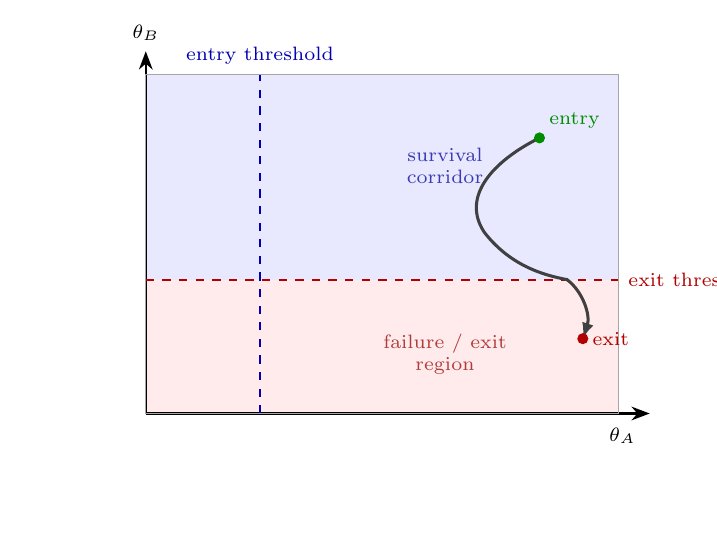
\begin{tikzpicture}[
  font=\sffamily,
  >=Stealth,
  axis/.style={->, line width=0.8pt},
  thresh/.style={dashed, line width=0.7pt},
  pathline/.style={draw=black!75, line width=1.1pt, -{Latex[length=2mm]}},
  lab/.style={font=\scriptsize, align=center},
  regionlab/.style={font=\scriptsize, align=center, text opacity=0.75}
]
\path[use as bounding box] (-0.7,-0.7) rectangle (7.7,5.4);

\fill[blue!9] (0.8,1.2) rectangle (6.8,4.8);
\fill[red!8] (0.8,0.5) rectangle (6.8,2.2);
\draw[axis] (0.8,0.5) -- (7.2,0.5) node[below left=2pt, lab] {$\theta_A$};
\draw[axis] (0.8,0.5) -- (0.8,5.1) node[above, lab] {$\theta_B$};
\draw[black!35] (0.8,0.5) rectangle (6.8,4.8);

\draw[thresh, blue!70!black] (2.25,0.5) -- (2.25,4.8)
  node[above, lab, text=blue!70!black] {entry threshold};
\draw[thresh, red!70!black] (0.8,2.2) -- (6.8,2.2)
  node[right, lab, text=red!70!black] {exit threshold};

\node[regionlab, text=blue!60!black] at (4.6,3.65) {survival\\corridor};
\node[regionlab, text=red!60!black] at (4.6,1.25) {failure / exit\\region};

\draw[pathline]
  (5.8,4.0)
  .. controls (5.2,3.7) and (4.8,3.25) .. (5.1,2.8)
  .. controls (5.45,2.35) and (5.9,2.25) .. (6.15,2.2)
  .. controls (6.35,2.05) and (6.45,1.75) .. (6.35,1.45);
\fill[green!55!black] (5.8,4.0) circle (2pt) node[above right, lab] {entry};
\fill[red!70!black] (6.35,1.45) circle (2pt) node[right, lab] {exit};
\end{tikzpicture}
\end{document}
